\documentclass[sutton_barto_notes.tex]{subfiles}

\begin{document}


\newpage
\section{Finite Markov Decision Processes}

\mybox{\textsc{When you’re presented with a problem in industry, the first and most important step is to translate that problem into a Markov Decision Process (MDP). The quality of your solution depends heavily on how well you do this translation.}}

\begin{definition}
finite Markov Decision Processes, involves evaluative feedback (as in bandits) and associative settings (choosing different actions in different situations)
\end{definition}

MDPs are a classical formalization of \textit{sequential} decision making, where actions influence both immediate rewards and subsequent states (thus influence future/delayed rewards as well). MDPs need to consider trade-off between immediate reward and delayed reward.

In bandit problems, we estimated the value $q_{*}(a)$ of each action $a$.

In MDPs, we estimate $q_{*}(s,a)$ (value of each action $a$ in each state $s$), or $v_{*}(s)$ (value of each state given optimal action selections).

MDPs are an ideal form of the RL problem where precise theoretical statements can be made.
Key elements of RL's mathematical structure: returns, value functions, and Bellman equations.

\subsection{The Agent-Environment Interface}

\begin{itemize}
\item agent: learner and decision maker
\item environment: everything outside the agent, and which agent interacts with
\end{itemize}

\begin{figure}[!h]
  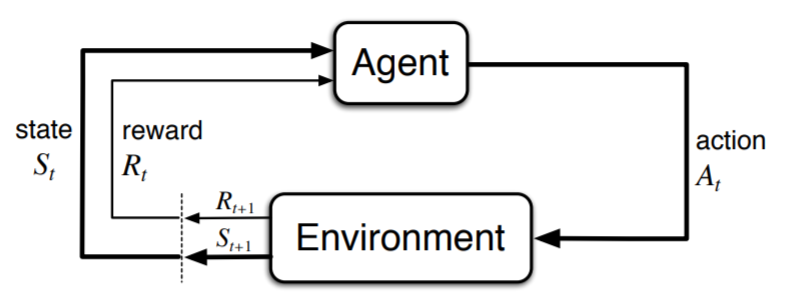
\includegraphics[width=\linewidth]{MDP_interface.PNG}
  \caption{The agent-environment interaction in a MDP}
  \label{fig:MDP_interface}
\end{figure}

At each time step $t$, the agent receives some representation of the environment's $state$, $S_t$, and on the state selects an $action$, $A_t$. One time step later, the agent receives reward $R_{t+1}$ as a result of the action, and find itself in a new state $S_{t+1}$. The trajectory/sequence is:

$$ S_0, A_0, R_1, S_1, A_1, R_2, S_2, A_2, R_3, \cdots $$

In a \textit{finite} MDP, the state sets, action sets and reward sets are finite.

Following defines the \textit{dynamics} of the MDP.

$$ p(s', r| s, a) \doteq P(S_t = s', R_t = r | S_{t-1} = s, A_{t-1} = a) $$
$$ \sum_{s' \in \mathcal{S}} \sum_{r \in \mathcal{R}} p(s',r|s,a) = 1, \forall s \in \mathcal{S}, a \in \mathcal{A}(s) $$

$p$ specifies a probability distribution for each choice of $s$ and $a$.
The probability of each possible value for $S_t$ and $R_t$ depends on the immediately preceding state and action, $S_{t-1}$ and $A_{t-1}$ (note not including earlier states and actions).

\begin{definition}
Markov property\footnote{Markov property refers to the memoryless property of a stochastic process. "only present matters"}, the future only depends on the current state, not the history.
\end{definition}

\begin{definition}
state-transition probabilities,
$$ p(s'|s,a) \doteq P(S_t=s'|S_{t-1}=s, A_{t-1}=a) = \sum_{r\in \mathcal{R}} p(s',r|s,a) $$
\end{definition}
We can express state transition probabilities in an Matrix as shown in Figure \ref{fig:state-trans-prob-eg}. Each row in the matrix represents the probability from moving from our original state to any successor state. Sum of each row is equal to 1.
\begin{figure}[h!]
  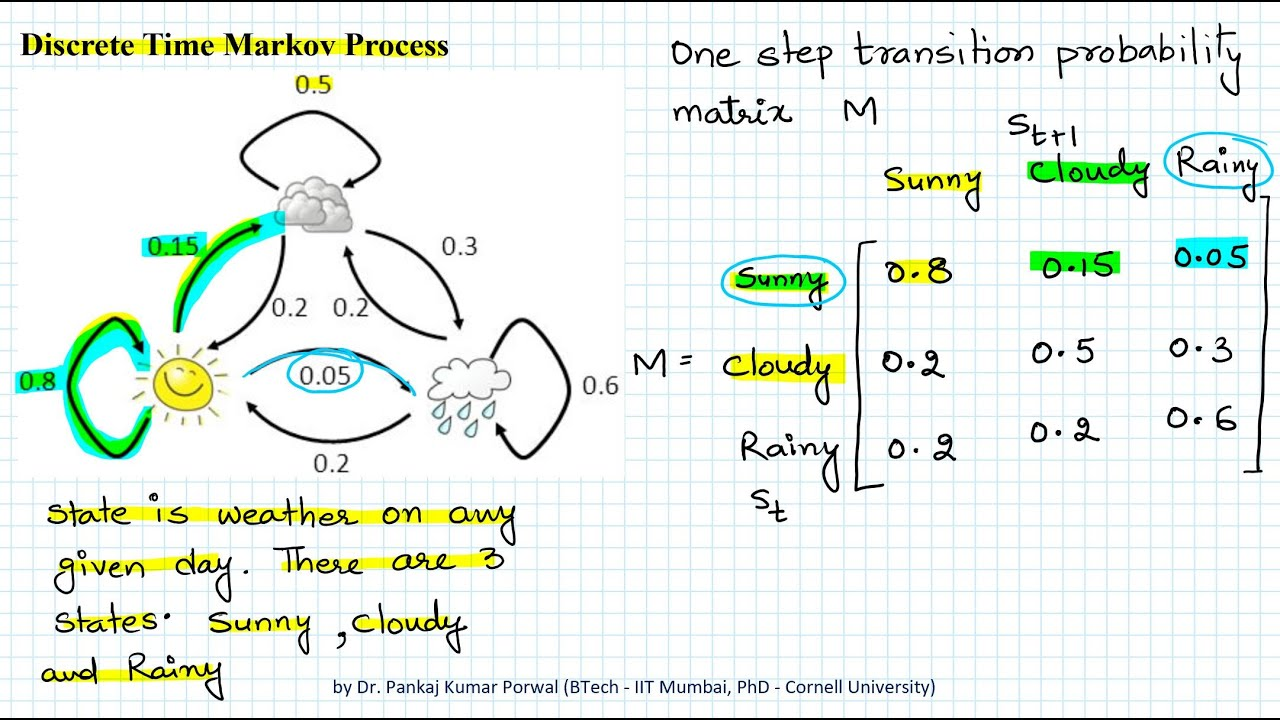
\includegraphics[width=\linewidth]{state_transition_probability_example.jpg}
  \caption{An example of state transition probability.}
  \label{fig:state-trans-prob-eg}
\end{figure}

\begin{figure}[h!]
  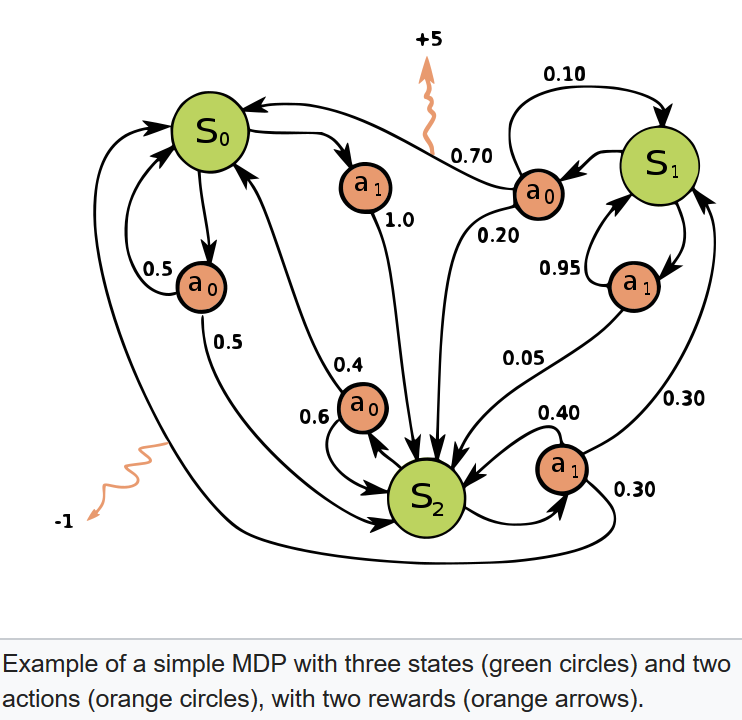
\includegraphics[width=0.7\linewidth]{state_transition_probability_example_2.png}
  \caption{A complex example of state transition probability.}
  \label{fig:state-trans-prob-eg2}
\end{figure}

\begin{definition}
expected rewards for state-action pairs

$$ r(s,a) \doteq \E [R_t | S_{t-1}=s, A_{t-1}=a] = \sum_{r\in \mathcal{R}} r \sum_{s\in \mathcal{S}} p(s',r|s,a) $$
\end{definition}

\begin{definition}
expected rewards for state-action-nextState,

$$ r(s,a,s') \doteq \E [R_t | S_{t-1}=s, A_{t-1}=a, S_t=s'] = \sum_{r \in \mathcal{R}} r \frac{p(s',r|s,a)}{p(s'|s,a)} $$
\end{definition}

\textbf{Question}: Why does the definition of the reward function $r(s,a,s')$ involve the term $p(s'|s,a)$? \url{https://ai.stackexchange.com/q/20244/55308}

Expectation of reward after taking action $a$ in state $s$ and ending up in state $s'$ would be:
$$ r(s,a,s') \doteq \sum_{r\in \mathcal{R}} r \cdot p(r|s,a,s') $$
Since we do not define $p(r|s,a,s')$, we have following equation with product rule:
$$ p(s',r|s,a) = p(s'|s,a) \cdot p(r|s',s,a) $$
After moving $p(s'|s,a)$ to the LHS, we see that:
$$ r(s,a,s') \doteq \sum_{r \in \mathcal{R}} r \frac{p(s',r|s,a)}{p(s'|s,a)} $$



\paragraph{agent-environment}
The agent-environment boundary represents the lit of the agent's absolute control, not of its knowledge. Anything that cannot be changed by the agent.

Any problem of learning goal-directed behavior can be reduced to 3 signals passing back and forth between an agent and its environment:
\begin{itemize}
\item action: the choice made by the agent
\item the basis on which the choice is made
\item the agent's goal
\end{itemize}

\begin{example}
Bioreactor,

\begin{itemize}
\item actions (vector): target temperatures, target stirring rates
\item states (vector): sensory readings, ingredients input, target chemical
\item rewards (number): production rate of useful chemical (target)
\end{itemize}

\end{example}

\begin{example}
Robotic Arm (pick-and-place task)

\begin{itemize}
\item actions: voltages applied to each joint motor
\item states: readings of joint angles and velocities
\item rewards: +1 for successfully object pick-and-place; small negative reward at each time step (punish jerkiness motion)
\end{itemize}
\end{example}


\subsection{Goals and Rewards}
 In RL, the purpose/goal of the agent is to maximize \textit{cumulative reward in the long run}.
 It is important that the set-up rewards indicate what we truly want accomplished.
 In particular, rewards are not the place to tell/impart agent prior knowledge about \textit{how} to achieve our goal.
 For example, in a chess game, the agent should only be reward for winning, instead of achieving subgoals like taking opponent's pieces.
 Better places for imparting this kind of prior knowledge in (1) initial policy; or (2) initial value function.
 
The reward signal is a way of imparting to the agent \textit{what} you want achieved, not \textit{how} you want it achieved.

\textbf{reward hypothesis}: That all of what we mean by goals and purposes can be well thought of as the maximization of the expected value of the cumulative sum of a received scalar signal (reward).

\subsection{Returns and Episodes}

A RL agent's goal is to maximize the cumulative reward it receives in the long run.
In general, we seek to maximize the \textit{expected return} $G_t$.

$$ G_t \doteq R_{t+1} + R_{t+2} + \cdots + R_T $$

where $T$ is a final time step.

The final time step marks the end of a subsequences.

\begin{definition}
Episode, a subsequence of the agent-environment interaction. Each episode ends in \textbf{terminal state}, followed by a \textbf{reset} to a standard starting state or to a \textbf{sample} from a standard distribution of starting states. The next episode begins independently of how the previous one ended.
\end{definition}

The set of all nonterminal states, $\mathcal{S}$. All states and the terminal state, $\mathcal{S^+}$.

\begin{definition}
Episodic tasks, tasks with episodes that with terminal state.
\end{definition}

\begin{definition}
continuing tasks, tasks without terminal state.
\end{definition}

This task uses discounted rewards to deal with $T=\infty$.

\begin{definition}
discounted rewards $G_t$. discount rate, $0 \leq \gamma \leq 1$

$$ G_t \doteq R_{t+1} + \gamma R_{t+2} + \gamma^2 R_{t+3} + \cdots = \sum_{k=0}^{\infty} \gamma^k R_{t+k+1} $$
\end{definition}

The discount rate determines the present value of future rewards. As long as the reward sequence {$R_k$} is bounded, the infinite sum $G_t$ has a finite value.
If $\gamma \rightarrow 0$, the agent is myopic; if $\gamma \rightarrow 1$, the agent is farsighted.

If the reward is constant $R$, then we have the \textit{geometric series}

$$ G_t = \sum_{k=0}^{\infty} R\gamma^k = R\frac{1}{1-\gamma} $$

Note that the returns at successive time steps are related to each other (which is important for RL):

$$ G_t \doteq R_{t+1} + \gamma R_{t+2} + \gamma^2 R_{t+3} + \cdots = R_{t+1} + \gamma G_{t+1} $$

\begin{example} pole-balancing
\begin{itemize}
\item terminal state: if the pole falls past a given angle from vertical or if the cart runs off the track
\item starting state: pole reset to vertical
\item reward (episodic): +1 for each time step before falling
\item reward (continuing): -1 on each falling, 0 for all other times
\end{itemize}
\end{example}


\begin{figure}[!h]
  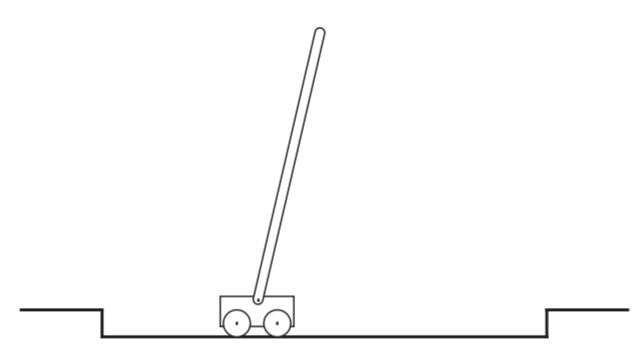
\includegraphics[width=\linewidth]{MDP_pole.PNG}
  \label{fig:MDP_pole}
\end{figure}



\subsection{Unified Notation for Episodic and Continuing Tasks}

We use $S_{t,i}$ to represents state at time $t$ of episode $i$ (same for $A_{t,i}$, $R_{t,i}$, etc).
In practice, we dropped the $i$ as we normally don't have to distinguish between different episodes.
So, now $S_t$ refers to $S_{t,i}$.

We use an $absorbing state$ to replace the terminate state. The absorbing state transits to itself and have reward = 0.
This way, we can have the same formula of $G_t$ for episodic and continuing tasks.

\subsection{Policies and Value Functions}

Value functions (either V or Q) are \textbf{always} conditional on some policy $\pi$. Sometimes in literature we leave off the $\pi$ or $*$ and just refer to $V$ and $Q$, because it is implicit in the context, but ultimately, every value function is always with respect to some policies.

\begin{definition}
There are two value functions:
\begin{itemize}
\item value functions of states, or V, estimate how much expected return it is received for the agent to be in a given state;
\item value functions of state-action pairs, or Q, estimate how much expected return it is received to perform a given action in a given state.
\end{itemize}
\end{definition}

\begin{definition}
policy, $\pi(A_t=a|S_t=s)$, a mapping from states to probabilities of selecting each action. In other words, policy is a distribution over actions for each possible state.
\end{definition}
\begin{itemize}
\item deterministic policy: map each state to an action. $\pi(s)$. 
\item stochastic policy: map each state to a distribution over all possible actions. $\pi(a|s)$
\end{itemize}
Valid policy can \textbf{only} depend on current state, not other things like time or previous state (if, for example, last action affect rewards heavily, then the last action must include in the states). 
\newline

Expectation of $R_{t+1}$ in terms of $\pi$ and the four-argument function $p$:
\[
\E\left[R_{t+1} \middle|S_{t}\right] = \sum_{a \in \mathcal{A}} \pi\left(a \middle| S_t\right) \cdot r(S_t, a) = \sum_{a \in \mathcal{A}} \pi\left(a \middle| S_t\right) \cdot \sum_{r \in \mathcal{R}} r \sum_{s' \in \mathcal{S}} p\left(s', r \middle| S_t, a\right)
\]
My word explanation: the expectation of reward given current state $S_t$= the total sum of the probability of perform action $a$ at state $s$ $\cdot$ the reward $r$ $\cdot$ the probability of getting reward $r$ (when performs action $a$ at state $s$) (?)

\begin{definition}
state-value function for policy $\pi$, (value function of a state $s$ under a policy $\pi$), $v_{\pi}(s)$, is the expected return when starting in $s$ and following $\pi$ thereafter. For MDPs:

$$ v_\pi(s) \doteq \E_\pi[G_t | S_t = s] = \E_\pi [ \sum_{k=0}^{\infty} \gamma^k R_{t+k+1} | S_t = s], \forall s \in \mathcal{S} $$
\end{definition}

\begin{definition}
action-value function for policy $\pi$, (value of taking action $a$ in state $s$ under a policy $\pi$), $q_\pi(s,a)$, is the expected return starting from $s$, taking the action $a$, and \textbf{then} following policy $\pi$:

$$ q_\pi(s,a) \doteq \E_\pi [G_t | S_t = s, A_t = a] = \E_\pi [\sum_{k=0}^{\infty} \gamma^k R_{t+k+1} | S_t = s, A_t = a] $$
\end{definition}

The main difference between $Q$ and $V$ then, is the $Q$-value lets you play a hypothetical of potentially taking a different action in the first time step than what the policy might prescribe and then following the policy from the state the agent winds up in.

The value functions enable us to judge the quality of a policy.
\newline

Equation of $v_\pi$ in terms of $q_\pi$ and $\pi$:
$$ v_\pi(s) = \sum_a \pi(a|s)q_\pi(s,a) $$

My word explanation: the value function is the total sum of probability of choosing action $a$ at state $s$ $\times$ the action-value of taking each action.
\newline
Equation of $v_\pi$ in terms of $\pi$ and $p$:
\begin{align*}
v_\pi(s) & \doteq \E_\pi[G_t | S_t = s]\\
& = \E_\pi[R_{t+1} + \gamma G_{t+1} | S_t = s]\\
& = \sum_a \pi(a|s) \sum_{s'}\sum_r p(s',r|s,a) [r+ \gamma \E_\pi[G_{t+1} | S_{t+1}=s']]\\
& = \sum_a \pi(a|s) \sum_{s',r} p(s',r|s,a) [r+ \gamma v_\pi(s')]
\end{align*}

Equation of $q_\pi$ in terms of $v_\pi$ and the four argument $p$
$$ q_\pi(s,a) = \sum_{s', r} p(s',r|s,a) \underbrace{ [r+\gamma v_\pi(s')] }_{G_t?} $$

\begin{definition}
Monte Carlo methods, estimation methods that involve averaging over many random samples of actual returns.
\end{definition}

For example, an agent follows policy $\pi$; and for each state $s$, the agent maintains an average of the actual returns which have followed that state, then the average converges to the state's value $v_\pi(s)$. (Recall the Law of Large Numbers, or sample-average method in Chapter 2).
For another example, if separate averages are kept for each action taken in each state, then these averages will similarly converge to the action values $q_\pi(s,a)$.

\begin{definition}
Bellman equation for $v_\pi$:

$$ v_\pi = \sum_a \pi(a|s) \sum_{s',r} p(s',r|s,a) [r+ \gamma v_\pi(s')] $$
\end{definition}

It expresses a relationship between the value of a state and the values of its successor states. First, we expand the expected return as a sum over possible action choices made by the agent. Second, we expand over possible rewards and next states condition on state $s$ and action $a$. We break it down in this order because the action choice depends only on the current state, while the next state and reward depend only on the current state and action. 

\begin{figure}[!h]
  \centering
  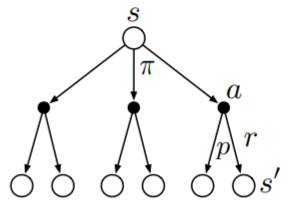
\includegraphics[]{MDP_backup.PNG}
  \caption{Backup diagram for $v_\pi$}
  \label{fig:MDP_backup}
\end{figure}
Note that in backup diagram, the nodes do not necessarily represent distinct states (e.g. a state might be its own successor).

The value function $v_\pi$ is the unique solution to its Bellman equation (??). My understanding is that since $v_\pi$ is the only solution, meaning that $v_\pi$ must converge to a point?

\begin{definition}
Bellman equation for $q_\pi$:

$$ q_\pi(s,a) \doteq \E_\pi [G_t | S_t = s, A_t = a] = \sum_{s',r} p(s',r|s,a)[r+\gamma \sum_{a'} \pi(a'|s')q_\pi (s',a')] $$
\end{definition}

\begin{figure}[!h]
  \centering
  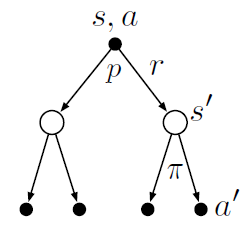
\includegraphics[]{MDP_backup_Qpi.PNG}
  \caption{Backup diagram for $q_\pi$}
  \label{fig:MDP_backup_qpi}
\end{figure}

\begin{figure}[!h]
    \centering
    \subfigure[]{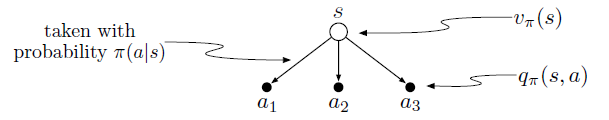
\includegraphics[width=\textwidth]{MDP_1.PNG}}
    \subfigure[]{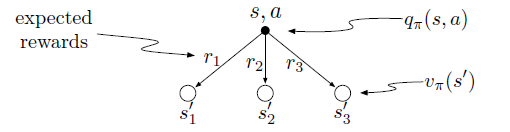
\includegraphics[width=\textwidth]{MDP_2.PNG}}
    \caption{ (a) $ v_\pi(s)=\sum_a \pi(a|s)q_\pi(s,a) $ (b) $ q_\pi(s,a)=\sum_{s',r}p(s',r|s,a)[r+\gamma v_\pi(s')] $ }
    \label{fig:MDPMDP}
\end{figure}
The value of a state depends on the values of the actions possible in that state and on how likely each action is to be taken under the current policy.

We can use the Bellman Equation to solve for a value function by writing a system of linear equations. However, we can only solve small MDPs directly, but Bellman Equations will factor into the solutions we see later for large MDPs.

\subsection{Optimal Policies and Optimal Value Functions}

Solving a RL means finding a policy that achieves a lot of reward over the long run.

\begin{definition}
optimal policy, $\pi_*$

$$ \pi_* \geq \pi' \iff v_\pi(s) \geq v_{\pi'}(s), \quad \forall s \in \mathcal{S} $$
\end{definition}
An optimal policy is defined as the policy with the highest possible value function in all states. At least one (deterministic) optimal policy always exists, but there may be more than one. The exponential number of possible policies makes searching for the optimal policy by brute-force intractable.

\begin{definition}
optimal state-value function, $v_*$

$$ v_*(s) \doteq \max_\pi v_\pi(s), \quad \forall s \in \mathcal{S} $$
\end{definition}

\begin{definition}
optimal action-value function, $q_*$

$$ q_*(s) \doteq \max_\pi q_\pi(s,a), \quad \forall s \in \mathcal{s}, a \in \mathcal{A} $$
\end{definition}

We can write $q_*$ in terms of $v_*$:

$$ q_*(s,a) = \E [R_{t+1} + \gamma v_* (S_{t+1}) | S_t = s, A_t = a] $$

\begin{definition}
Bellman optimality equation for $v_*$,
\begin{align*}
v_*(s) &= \sum_a \pi_* (a|s) q_{\pi_*} (s,a) \\
& = \max_{a\in\mathcal{A}}(s) q_{\pi_*} (s,a) \\
& = \max_a \E [R_{t+1} + \gamma v_* (S_{t+1}) | S_t = s, A_t = a] \\
& = \max_a \sum_{s',r} p(s',r|s,a)[r+\gamma v_*(s')]
\end{align*}
\end{definition}

\begin{definition}
Bellman optimality equatoin for $q_*$,
\begin{align*}
q_*(s,a) & = \E [R_{t+1} + \gamma \max_{a'} q_*(S_{t+1}, a') | S_t = s, A_t = a] \\
& = \sum_{s',r} p(s',r|s,a)[r+\gamma \max_{a'} q_*(s',a')]
\end{align*}
\end{definition}

\begin{figure}[!h]
  \centering
  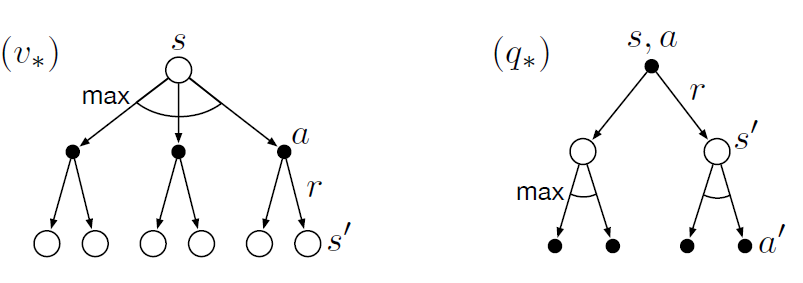
\includegraphics[]{MDP_optimal.PNG}
  \caption{Backup diagram for $v_*$ and $q_*$}
  \label{fig:MDP_optimal}
\end{figure}

$v_*$ is equal to the maximum of the term $\sum_{s',r} p(s',r|s,a)[r+\gamma v_*(s')]$ over all actions, while $\pi_*$ is the particular action achieves the maximum.
\newline

Explicitly solving the Bellman optimality equation provides one route to finding $\pi_*$, and thus to solving the RL problem.
However, this solution is rarely useful.
On one hand, $max_a$ is non-linear, so we cannot form linear equations as for Bellman equation.
On the other hand, it needs an exhaustive search, looking ahead at all possibilities, computing their probabilities of occurrence and their desirabilities in terms of expected rewards.
This solution relies on at least 3 assumptions:
\begin{itemize}
\item the dynamics of the environment are accurately known
\item computational resources are sufficient
\item the states have the Markov property
\end{itemize}

In RL, one typically has to settle for approximate solutions. Many RL methods can be taken as \textit{approximately} solving the Bellman optimality equation.

\paragraph{Exercise} Consider the contining MDP shown, the only decision to be made is in the top state with two actions (left, right).
Find optimal policy when $\gamma$ = 0.9.

\begin{figure}[!h]
  \centering
  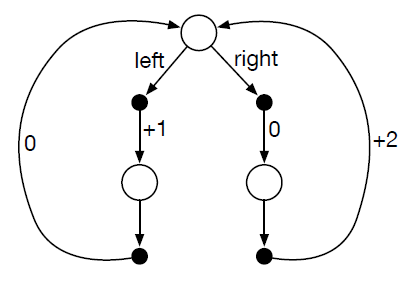
\includegraphics[width=0.2\linewidth]{ex3-22.PNG}
  \label{fig:ex3-22}
\end{figure}

\textbf{Solution}: Recall the definition of $v_\pi(s)$ and $q_\pi(s)$, we get

\begin{table}[h!]
\begin{tabular}{p{0.4\textwidth}p{0.4\textwidth}}
Left Policy & Right Policy \\
\begin{itemize}
\item $ v(s_0) = 1 + 0.9\cdot v(s_L) $
\item $ v(s_L) = 0 + 0.9\cdot v(s_0) $
\item $ v(s_R) = 2 + 0.9\cdot v(s_0) $
\end{itemize} & \begin{itemize}
\item $ v(s_0) = 0 + 0.9\cdot v(s_R) $
\item $ v(s_L) = 0 + 0.9\cdot v(s_0) $
\item $ v(s_R) = 2 + 0.9\cdot v(s_0) $
\end{itemize}  
\end{tabular}
\end{table}
Solving above we find that all state values of Right Policy is greater than all state values of Left Policy. Thus, `right' is the optimal policy for $\gamma$ = 0.9.

It is important to note that if we take `left' action in $s_0$, then policy $\pi$ would never take us to state $s_R$ (same for `right' and $s_L$); however, due to the definition of $\pi_*$, we must evaluate the value function for all states, even ones that would not be visited under a policy we are evaluating.

\begin{figure}[!h]
  \centering
  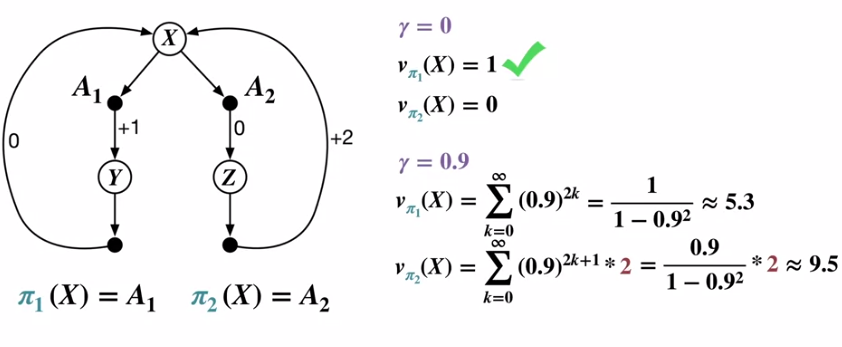
\includegraphics[width=\linewidth]{ex3-22-soln.png}
  \label{fig:ex3-22-soln}
\end{figure}
To explain the geometry series, the left is 1, $\gamma\cdot$0, $\gamma^2\cdot$1, $\gamma^3\cdot$0 sequence and the right is 0, $\gamma\cdot$2, $\gamma^2\cdot$0, $\gamma^3\cdot$2 sequence. Taking discounted sum into consideration, we have the geometry series.

\subsection{Optimality and Approximation}

It is difficult to reach optimal solutions due to constraints from computational resource and memory. We can often approximate the optimal solutions.

\subsection{Summary}

\begin{itemize}
\item RL is about learning from interaction how to behave in order to achieve a goal.
\item RL \textit{agent} and its \textit{environment} interact over a sequence of discrete time steps.
\item \textit{actions}: choices made by the agent, \textit{states}: the basis for making the choices, \textit{rewards}: basis for evaluating the choices.
\item everything inside agent is known and controllable; environment is incompletely controllable, and are partially known
\item a \textit{policy} is a stochastic rule that the agent selects actions as a function of states
\item agent's objective is to maximize reward it receives in the long run
\item when RL setup with agent, environment, states, actions, rewards, policy and formulated with well-defined transition probabilities it constitutes a Markov decision process (MDP)
\item a finite MDP is an MDP with finite state sets, action sets and reward sets.
\item \textit{return} is the function of future rewards that the agent seeks to maximize (in expected value)
\item undiscounted formulation is appropriate for \textit{episodic tasks}
\item discounted formulation is appropriate for \textit{\textbf{tabular} continuing tasks} (but not for approximate continuing tasks; see chap 10.3-4)
\item \textit{value functions} $v_\pi$ (state) and $q_\pi$ (state-action pair) are the expected return from that state/state-action under policy $\pi$
\item \textit{optimal value functions} $v_*$ and $q_*$ are the largest expected return by any policy
\item A policy whose value functions are optimal is an optimal policy
\item !! A MDP can have many optimal policies, but can have only one unique optimal value function ($v_*$ and $q_*$)
\item Any policy that is \textit{greedy} w.r.t $v_*$ and $q_*$ must be $\pi_*$
\item The Bellman optimality equations are special consistency conditions that the optimal value functions must satisfy
\item In RL most cases, their optimal solutions cannot be found but must be approximated in some way.
\end{itemize}

\newpage
\subsection{Learning Objectives (UA RL MOOC)}
1. Understand Markov Decision Processes (MDP)

MDP adds associative perspective to bandit problem, the actions affect not only immediate reward but also future rewards.
MDP consists of states, actions and rewards. MDP state must have Markov property (only present matters).

2. Describe how the dynamics of an MDP are defined

The dynamics of an MDP is the transition probability $p(s',r|s,a)$.

3. Understand the graphical representation of a Markov Decision Process
4. Explain how many diverse processes can be written in terms of the MDP framework

From my understanding, almost all real world problems can be written in MDP framework. The issue is that reward definition sometimes may not be accurate, and states, actions may not be finite.

5. Describe how rewards relate to the goal of an agent

The reward is a way of imparting to the agent what you want to achieved, not how you want to achieved.

6. Understand episodes and identify episodic tasks

Episodes have finite trajectory length and must end in a terminal state. Episodes are independent of previous episode.
Episodic task is task with episodes that ends in terminal state.

7. Formulate returns for continuing tasks using discounting

$$ G_t \doteq R_{t+1} + \gamma R_{t+2} + \gamma^2 R_{t+3} + \cdots = \sum_{k=0}^{\infty} \gamma^k R_{t+k+1} $$

8. Describe how returns at successive time steps are related to each other

$$ G_t = R_{t+1} + \gamma G_{t+1} $$

9. Understand when to formalize a task as episodic or continuing

When the tasks can be naturally broken into episodes (like chess game), the task is episodic; otherwise it is continuing task (like walking robot).

10. Recognize that a policy is a distribution over actions for each possible state

Policy is either a deterministic one (mapping from state to action) or a stochastic one (with probability distribution from state to actions).
The deterministic policy can be considered as a 100\% probability distribution policy.

11. Describe the similarities and differences between stochastic and deterministic policies

see 10

12. Generate examples of valid policies for a given MDP

13. Describe the roles of state-value and action-value functions in reinforcement learning

state-value gives the total expected return of a state following a policy, and action-value gives the total expected return of a state with an action then following a policy.
The scalar values (those expected returns) helps us to choose optimal policies, which solves an RL problem.

14. Describe the relationship between value functions and policies

Each value function are always associated with some policies. For example, the state value function:
$$v_\pi (s) = \sum_a \pi (a|s) \sum_{s',r} p(s',r|s,a)[r+\gamma v_\pi(s')] $$

15. Create examples of valid value functions for a given MDP

16. Derive the Bellman equation for state-value functions

\begin{align*}
v_\pi(s) & \doteq \E_\pi[G_t | S_t = s]\\
& = \E_\pi[R_{t+1} + \gamma G_{t+1} | S_t = s]\\
& = \sum_a \pi(a|s) \sum_{s'}\sum_r p(s',r|s,a) [r+ \gamma \E_\pi[G_{t+1} | S_{t+1}=s']]\\
& = \sum_a \pi(a|s) \sum_{s',r} p(s',r|s,a) [r+ \gamma v_\pi(s')]
\end{align*}

17. Derive the Bellman equation for action-value functions

$$ q_\pi(s,a) = \sum_{s', r} p(s',r|s,a) [r+\gamma v_\pi(s')] $$

18. Understand how Bellman equations relate current and future values

We see that current values (in LHS) and future values (in RHS) of the Bellman equations.

19. Use the Bellman equations to compute value functions

20. Define an optimal policy

$$ \pi_* \geq \pi' \iff v_\pi(s) \geq v_{\pi'}(s), \quad \forall s \in \mathcal{S} $$
An optimal policy is defined as the policy with the highest possible value function in all states.

21. Understand how a policy can be at least as good as every other policy in every state

Let us say there is a policy $\pi_1$ which does well in some states, while policy $\pi_2$ does well in others. We could combine these policies into a third policy $\pi_3$, which always chooses actions according to whichever of policy $\pi_1$ and $\pi_2$ has the highest value in the current state. $\pi_3$ will necessarily have a value greater than or equal to both $\pi_1$ and $\pi_2$ in every state.

22. Identify an optimal policy for given MDPs

23. Derive the Bellman optimality equation for state-value functions

\begin{align*}
v_*(s) &= \sum_a \pi_* (a|s) q_{\pi_*} (s,a) \\
& = \max_{a\in\mathcal{A}}(s) q_{\pi_*} (s,a) \\
& = \max_a \E [R_{t+1} + \gamma v_* (S_{t+1}) | S_t = s, A_t = a] \\
& = \max_a \sum_{s',r} p(s',r|s,a)[r+\gamma v_*(s')]
\end{align*}

24. Derive the Bellman optimality equation for action-value functions

\begin{align*}
q_*(s,a) & = \E [R_{t+1} + \gamma \max_{a'} q_*(S_{t+1}, a') | S_t = s, A_t = a] \\
& = \sum_{s',r} p(s',r|s,a)[r+\gamma \max_{a'} q_*(s',a')]
\end{align*}

25. Understand how the Bellman optimality equations relate to the previously introduced Bellman equations

26. Understand the connection between the optimal value function and optimal policies

27. Verify the optimal value function for given MDPs

28. Does adding a constant to all rewards change the set of optimal policies in episodic tasks? (Yes, adding a constant to all rewards changes the set of optimal policies.)
Does adding a constant to all rewards change the set of optimal policies in continuing tasks? (No, as long as the relative differences between rewards remain the same, the set of optimal policies is the same.)

\textbf{Explanation}: Let write $R_c$ for total reward with added constant $c$ of a policy as

$$ R_c = \sum_{i=0}^K (r_i + c) \gamma^i = \sum_{i=0}^K r_i \gamma^i + \sum_{i=0}^K c \gamma^i $$

So if we have two policies with the same total reward (w/o added $c$):

$$ \sum_{i=0}^{K_1} r_i^1\gamma^i = \sum_{i=0}^{K_2} r_i^2 \gamma^i $$

but with different lengths $K_1 \neq K_2$, the total reward with added constant will be different, because the second term in $R_c$ ($\sum_i^K c\gamma^i$) will be different.

For example, consider two optimal policies, both generating the same cumulative reward of 10, but the first policy visits 4 states before it reaches a terminal state, while the second visits only two states. The reward can be written as
$$ 10 + 0 + 0 + 0 = 10 $$
and
$$0+10=10$$
But when we add 100 to every reward:
$$ 110+100+100+100=410$$
and
$$100+110=210$$
Thus, now the first policy is better.

In the continuous case, the episodes always have length $K=\inf$. Therefore, they always have the same lenght, and adding a constant does not change anything, because the second term in $R_c$ stays the same.

29. $\gamma$ specifies the problem set. Once we have set the $\gamma$, we need to find the solution, so we do not want the agent to change the $\gamma$.

30. Adam: whenever I deal with continuous time system (like robotics), the first thing is: how do we discretize the time?

\end{document}